\documentclass{standalone}
\usepackage[dvipsnames]{xcolor}
\usepackage{pgfplots}
\pgfplotsset{
  compat=1.18, 
  trig format=rad, 
  ticklabel style = {font=\tiny},
  axis equal image,
}

\begin{document}
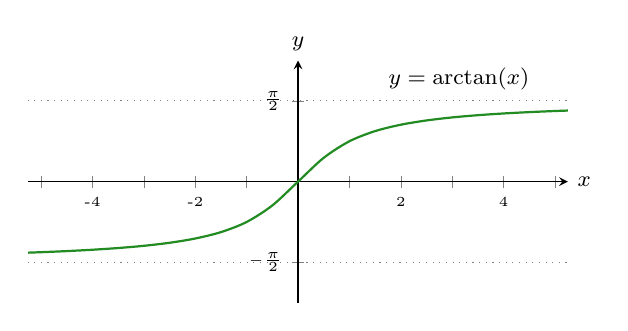
\begin{tikzpicture}
  \begin{axis}[
    xlabel={\footnotesize \(x\)},
    ylabel={\footnotesize \(y\)},
    ymin={-pi/2-pi/4},
    ymax={pi/2+pi/4},
    xmin={-5.25},
    xmax={5.25},
    axis x line={middle},
    axis y line={middle},
    xlabel style={at={(ticklabel* cs:1)}, anchor=west},
    ylabel style={at={(ticklabel* cs:1)}, anchor=south},
    xtick={-5, -4, -3, -2,-1,0,1, 2, 3, 4, 5},
    ytick={-3*pi/2, -pi, -pi/2, 0, pi/2, pi, 3*pi/2},
    xticklabels={,-4,,-2,,0,,2,,4,},
    yticklabels={,,\(-\frac{\pi}{2}\),,\(\frac{\pi}{2}\)},
    no marks
    ]

    % \addplot[thick, smooth, samples=1000, domain=-1:1] {asin(x)/180*pi};
    \addplot[ForestGreen, thick, smooth, domain=-6:6] {atan(x)};
    % \addplot[ForestGreen, smooth, dashed, domain={-pi-pi/2}:{-pi/2-0.1}] {atan(x)};
    % \addplot[ForestGreen, smooth, dashed, domain={pi/2}:{pi+pi/2-0.1}] {atan(x)};
    \addplot[dotted, gray] coordinates {(6,  -pi/2) (-6,  -pi/2)};
    \addplot[dotted, gray] coordinates {(6,   pi/2) (-6,   pi/2)};
    % \addplot[ForestGreen, thick, dotted, smooth, samples=1000, domain={-pi-pi/4}:{-pi/2}] {tan(x)};
    % \addplot[ForestGreen, thick, dotted, smooth, samples=1000, domain={pi/2}:{pi+pi/4}] {sin(x)};
    \node[right] at (pi/2,2) {\footnotesize \(y = \arctan(x)\)};
  \end{axis}
\end{tikzpicture}
\end{document}
